\chapter{Komponenten}
\label{chap:komponenten}

Bei den Recherchen der Projektarbeit hat sich die Erkenntnis ergeben, das eine erfolgreiche Verarbeitung von Anfragen die folgenden Komponenten benötigt:
\begin{itemize}
	\item Abbildung der Umwelt mittels Wissensdatenbank
	\item Definieren von Regeln zur Ableitung von Schlüssen mittels Logik
	\item Erkennung von Sprache in Schriftform
	\item Interne und externe Schnittstellen zur Kommunikation
\end{itemize}

Die oben genannten Komponenten werden bereits im Ansatz durch die in der Projektarbeit evaluierte Lösung --- Apache Stanbol --- zur Verfügung gestellt. Allerdings hat sich gezeigt, dass diese grössere Erweiterungen benötigen um die gewünschten Ergebnisse zu liefern.

\section{Architektur}
\label{sec:architektur}
Um die verschiedenen Teile zusammen zu nutzen, bietet Apache Stanbol eine frei konfigurierbare Verkettung dieser an. Dies geschieht mittels einer sogenannten Enhancement-Chain. Konkret heisst dies, dass eine beliebige Eingabe dieser Kette übergeben werden kann, worauf dann die erste Softwarekomponente der Kette die Eingabe verarbeitet und das Resultat an die nächste Komponente weiterreicht. Diese Vorgang wird durch sämtliche Komponenten der Kette fortgeführt bis schlussendlich das Endresultat an die anfragende Entität zurückgegeben wird.

Die Arbeit der Bachelorthesis besteht also darin, die Enhancement-Chain und die einzelnen Entitäten zu konfigurieren und zu erweitern.

%enhancementstructure.png/ https://stanbol.apache.org/docs/trunk/components/enhancer/enhancementstructure.png

\section{Abbildung der Umwelt mittels Wissensdatenbank}
\label{sec:architektur_wissensdatenbank}
\subsection{Objekte abbilden}
\label{subsec:architektur_wissensdatenbank_Objekte}
Die Abbildung der Umwelt geschieht in Apache Stanbol mittels dem sogenannten Entity Hub.
Dieser stellt Informationen zu Entitäten und Objekten einer spezifischen Wissensdomäne zur Verfügung. Die Beziehungen werden in Apache Stanbol in Form von Relationen zwischen den Entitäten abgebildet, analog dazu werden die Eigenschaften als Attribute erfasst. 

Die konkrete Arbeit mit dem Entity Hub besteht also darin Objekte, der für die Arbeit gewählten Domäne, als Entitäten abzubilden.

\subsection{Definieren von Regeln zur Ableitung von Schlüssen mittels Logik}
\label{sec:architektur_regeln}
Um nun aus der Wissensdatenbank Schlüsse ziehen zu können, werden Regeln benötigt. Regeln werden verwendet um mittels Bedingungen auf weitere Eigenschaften schliessen zu können.
Apache Stanbol unterstützt auf Prädikatenlogik basierende Regeln, welche innerhalb der Rule Store Komponente als Rezepte gespeichert werden. Diese sind nichts anderes als eine Zusammenfassung von Regeln, welche eine ähnliche Objektkategorie betreffen.

\section{Spracherkennung}
\label{sec:architektur_spracherkennung}
Um einen Eingabesatz auszuwerten, muss dieser erst als solcher erkannt werden. Konkret müssen also, die einzelnen Wörter als Tokens identifiziert und einer Sprachkategorie zugeorndet werden. Dies geschieht mittels der Spracheerkennungskomponente OpenNLP (open natural language processing). Diese Spracherkennung wird für die Englische Sprache von Stanbol schon weitgehend angeboten.

Nach unseren Erkenntinissen ist dies mit der Deutschen Sprache genau so möglich, jedoch nicht gegeben. Dies muss also noch erarbeitet werden. Nach ersten Recherchen wird dazu der Tokenizer sowie der Parser von \href{http://opennlp.sourceforge.net/models-1.5/}{OpenNLP} verwendet.

\section{Interne und Externe Schnittstellen zur Kommunikation}
\label{sec:architektur_schnittstellen}
Um die oben genannten Komponenten ansprechen und nutzen zu können, sind Schnittstellen zur Kommunikation unumgänglich.

\subsection{Interne Kommunikation}
\label{sec:architektur_schnittstellen_intern}
Intern nutzt Apache Stanbol, wie bereits beschrieben, die sogenannte Enhancement Chain um von einem gegebenen Input, mittels verschiedenen Komponenten, zu einem Output zu gelangen~\cite{stanbol:enhancementchain}. Die Enhancement Chain basiert auf einer Graph-Struktur, welche sie zur Kommunikation nutzt.

\begin{figure}[H]
	\centering
    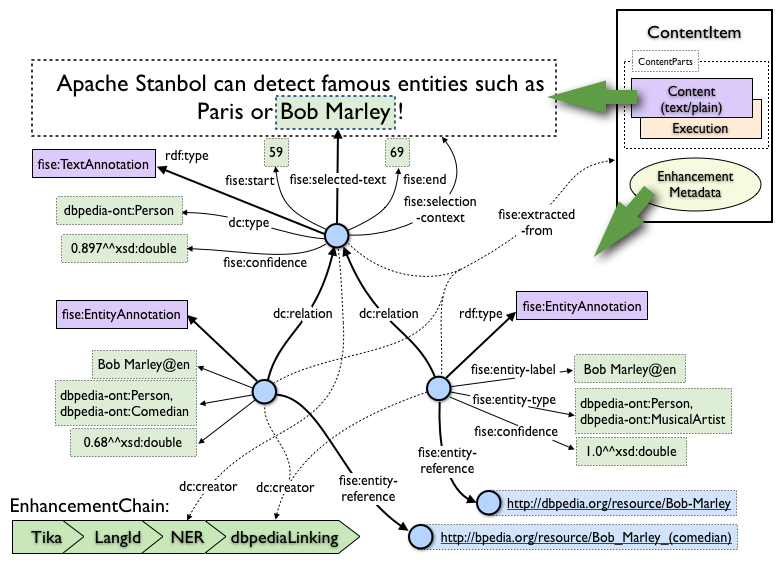
\includegraphics[scale=0.4]{bilder/enhancementstructure.png}
	\caption{Apache Stanbol Enhancement Chain\protect\footnotemark}
\label{fig:kommunikationKomponenten}
\end{figure}
\footnotetext{\cite{stanbol:enhancementgraph}}

\newpage

\subsection{Externe Kommunikation}
\label{sec:architektur_schnittstellen_extern}
Jede Komponente von Apache Stanbol, so z.B. auch die Enhancement Chain sowie deren Einzelkomponenten, verfügt über ein REST-Interface. Dies dient zur Kommunikation gegen aussen. Ein schematischer Ablauf der Kommunikation wird in Abbildung~\ref{fig:kommunikationKomponenten} grob dargestellt.

\begin{figure}[H]
	\centering
	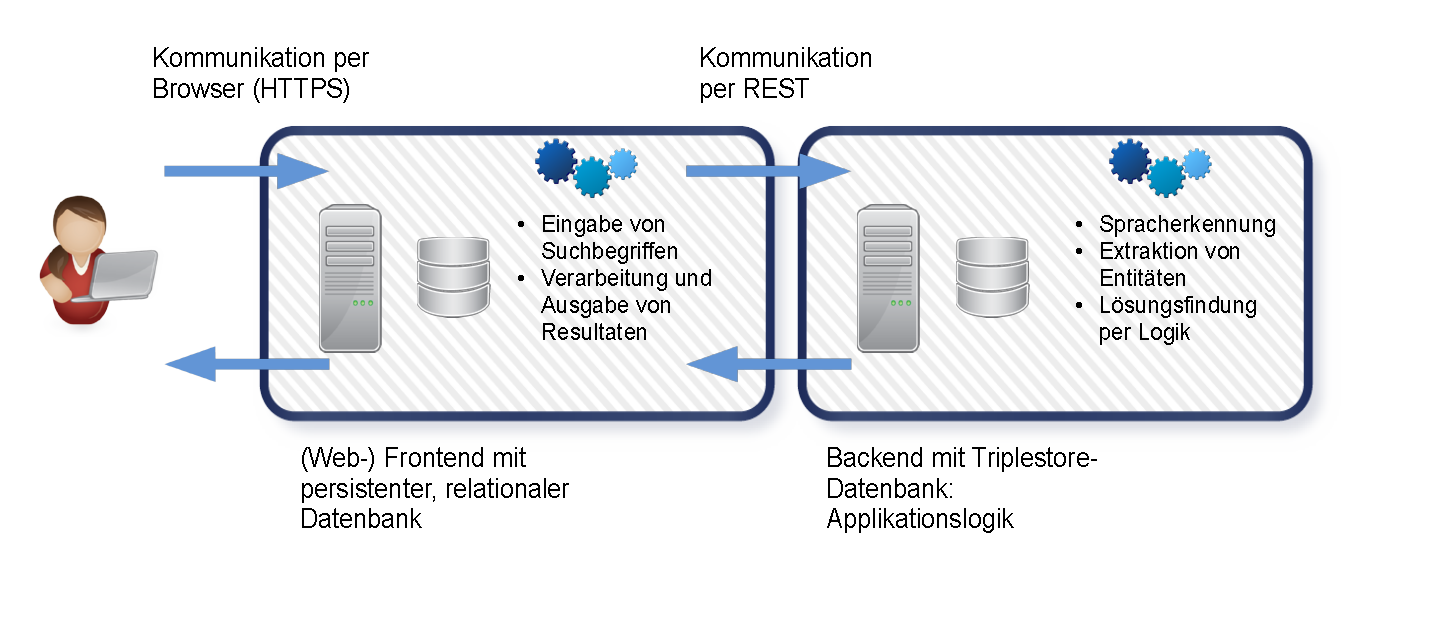
\includegraphics[scale=0.4]{bilder/software_komponenten.png}
	\caption{Kommunikation im Überblick\protect\footnotemark}
\label{fig:kommunikationKomponenten}
\end{figure}
\footnotetext{Eigene Darstellung mittels Libre Office Writer}
